\chapter{Mecánica: base, ruedas, brazo y pinza}\label{cap:mecanica}

\section{La base}

La base es una \textbf{caja de madera de 1~cm en forma de T}, de 40~cm de largo y unos 20~cm de alto (paredes de
18~cm), pintada de negro. Se definió en la entrega R2~E3.

\begin{itemize}
  \item \textbf{Adelante, la parte ancha}: 40 × 23~cm. Debajo van las dos ruedas locas.
  \item \textbf{Atrás, la parte angosta}: 34 × 17~cm, con las dos ruedas de tracción en rebajes de 3~cm a cada
        lado. Así las ruedas no sobresalen del ancho de la parte delantera.
  \item El origen de coordenadas del robot, \cod{base\_link}, está en el \textbf{eje de las ruedas de tracción}, a
        8,5~cm del borde trasero (figura~\ref{fig:planta}). $x$ apunta hacia adelante, $y$ a la izquierda y $z$ hacia
        arriba (convención REP-103 de ROS).
  \item Peso estimado del robot completo: 6--9~kg (la guía pide $\geq 5$~kg). \textbf{MEDIR}.
\end{itemize}

\begin{figure}[H]
\centering
\begin{subfigure}{0.36\textwidth}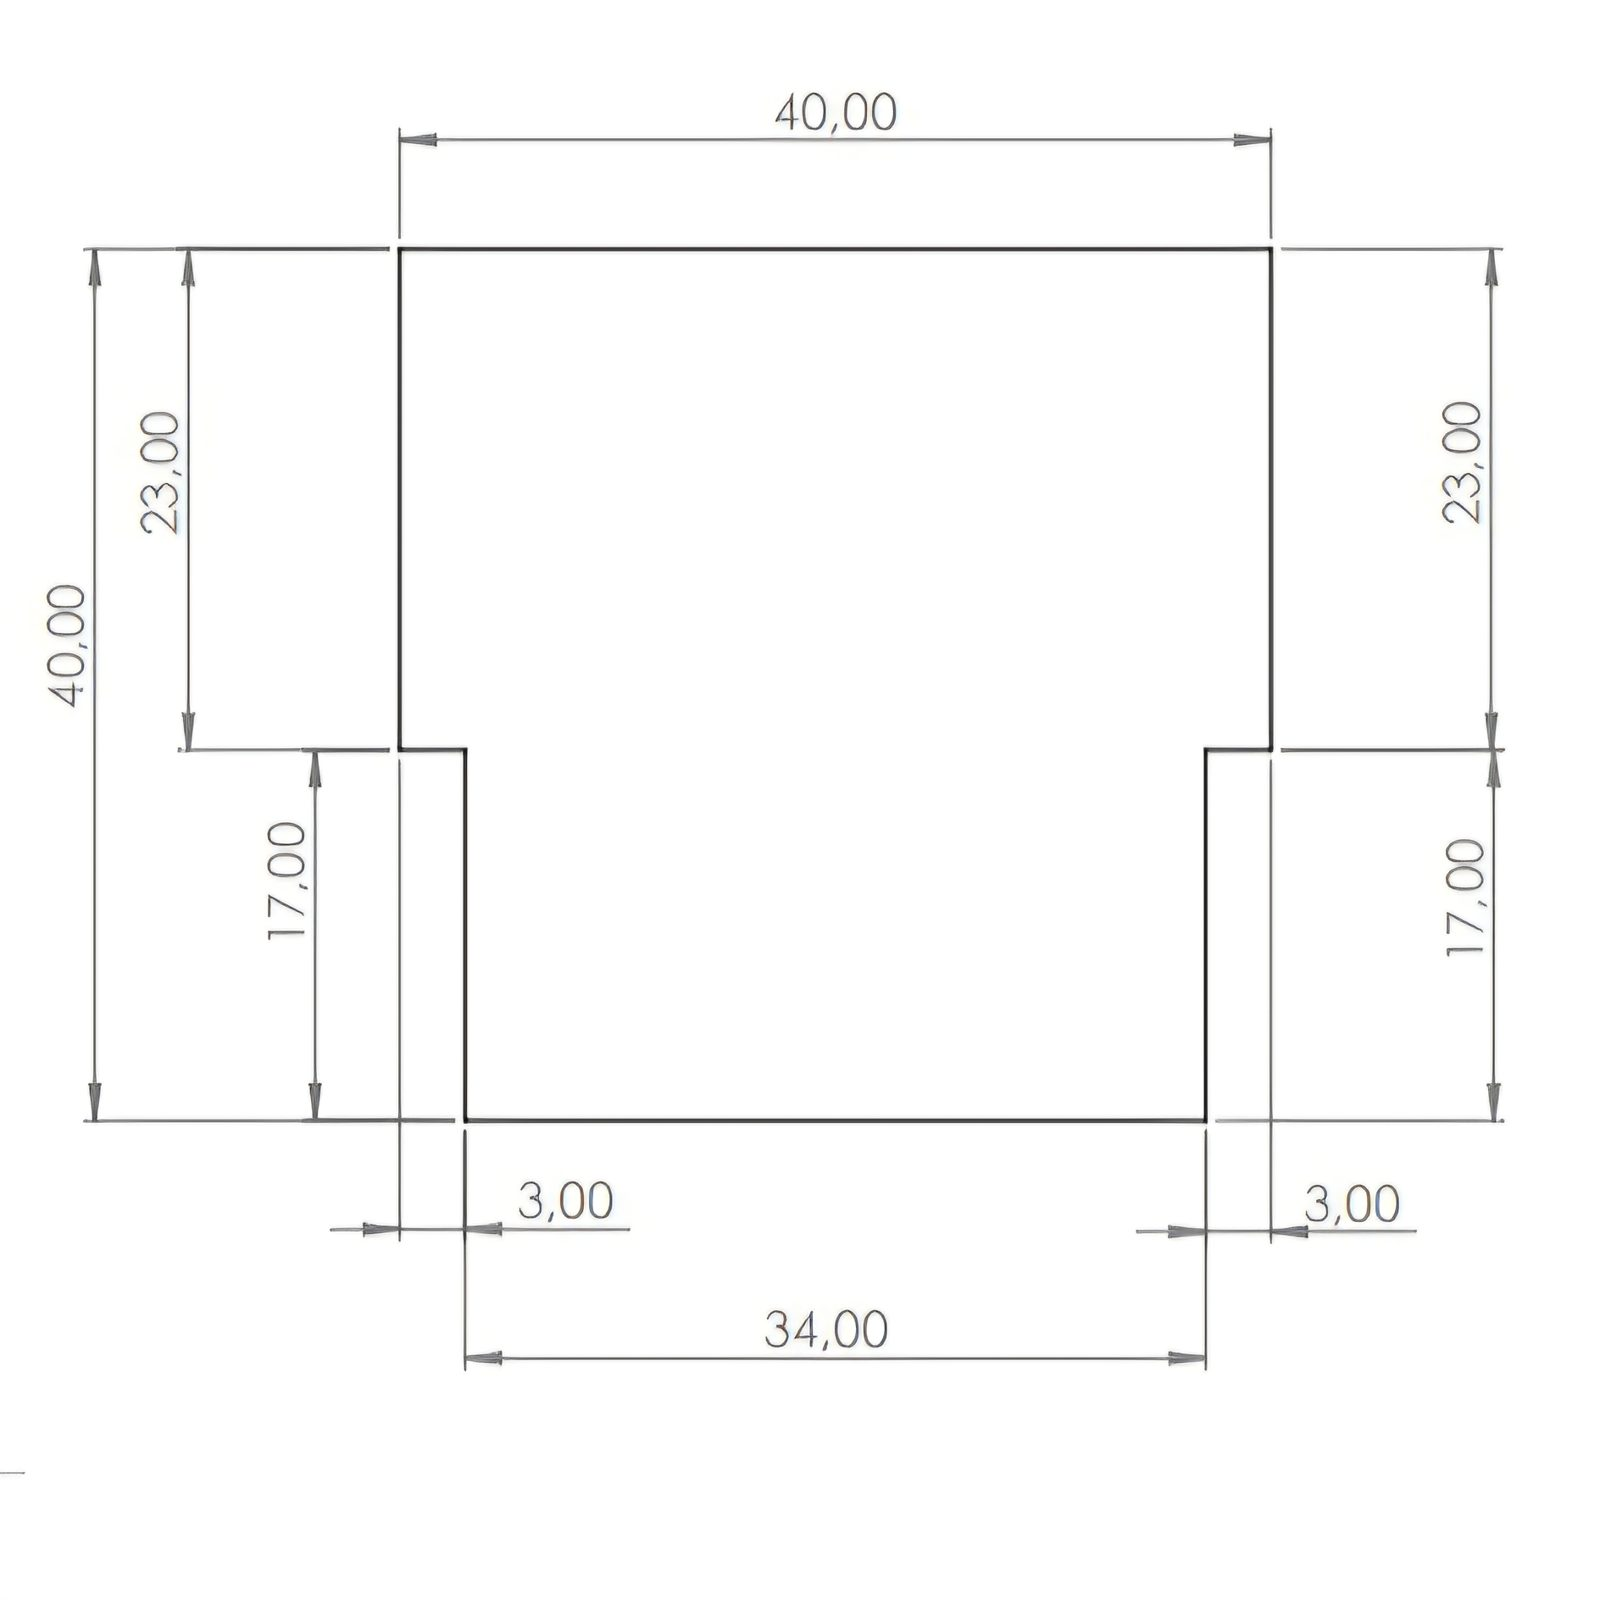
\includegraphics[width=\linewidth]{dimensiones_base.jpg}\caption{Planta de la tapa (cm).}\end{subfigure}\hfill
\begin{subfigure}{0.30\textwidth}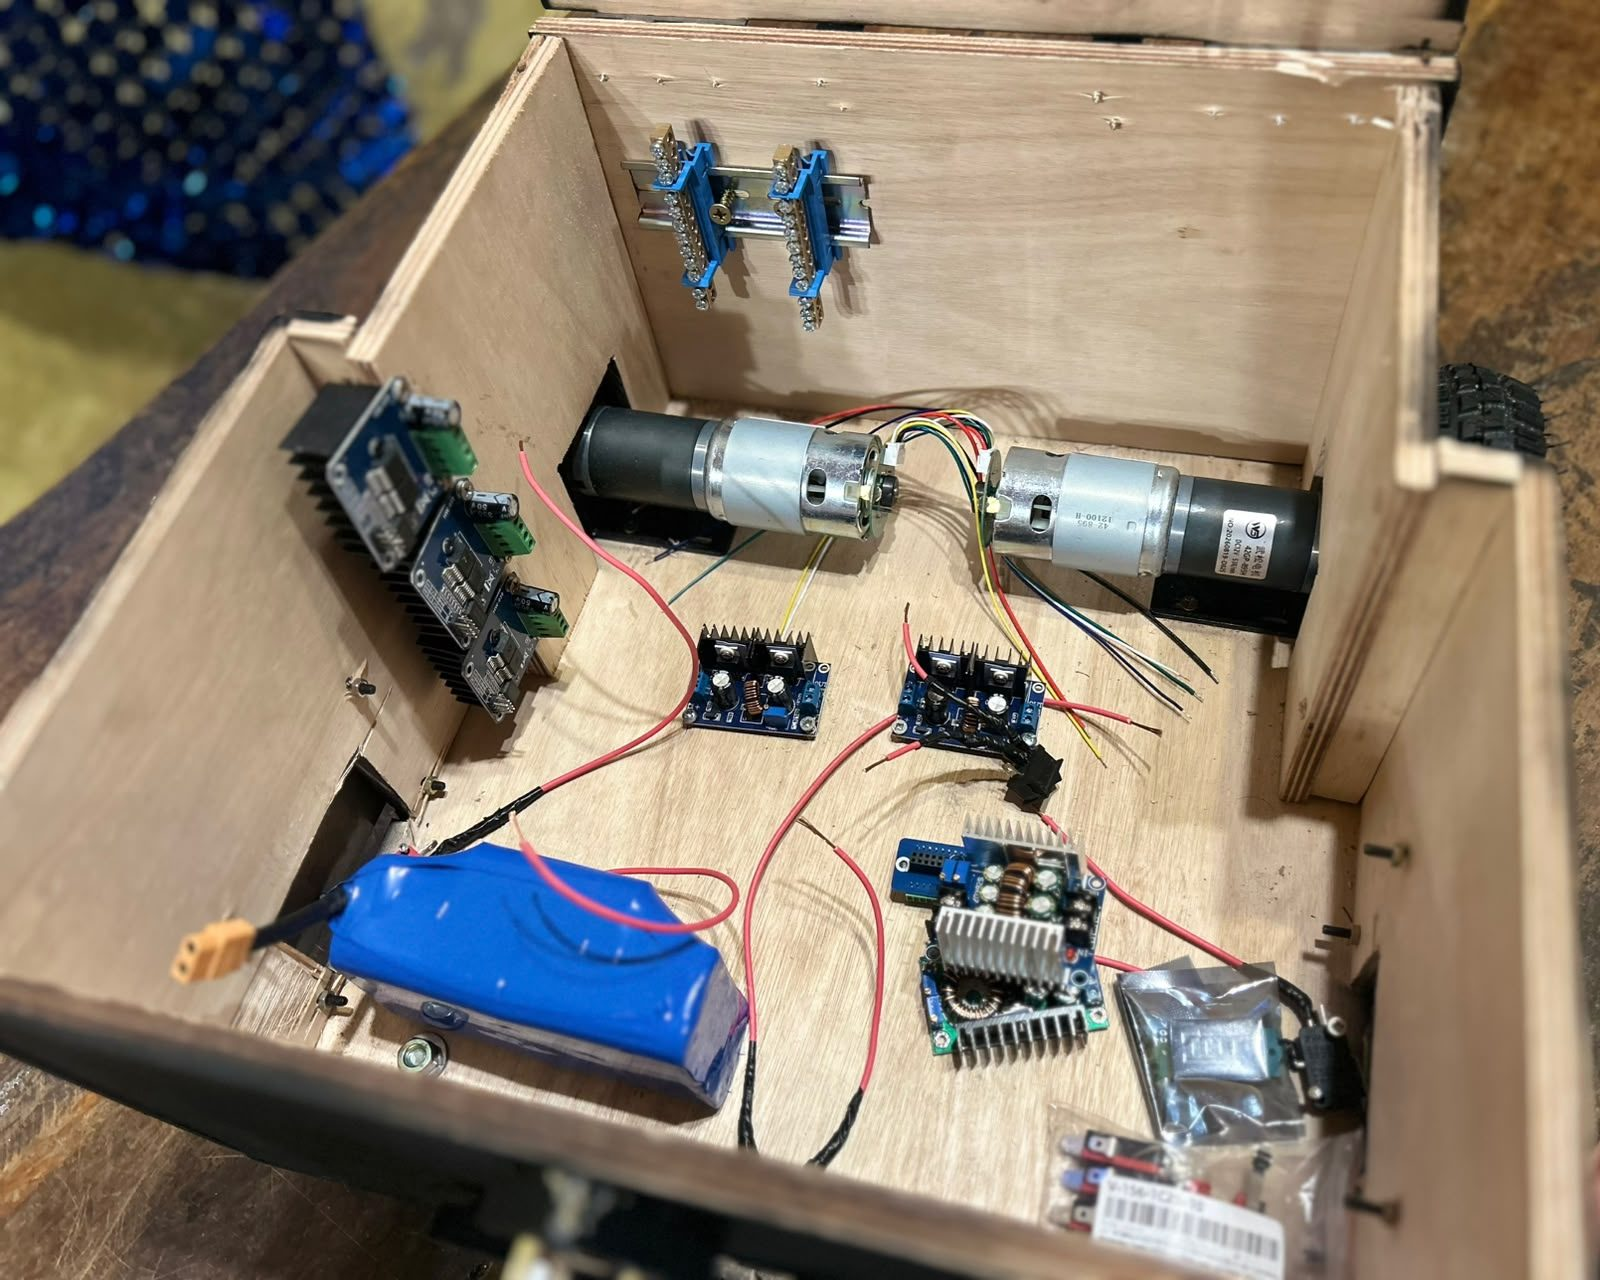
\includegraphics[width=\linewidth]{interior.jpg}\caption{Interior con la batería vieja.}\end{subfigure}\hfill
\begin{subfigure}{0.30\textwidth}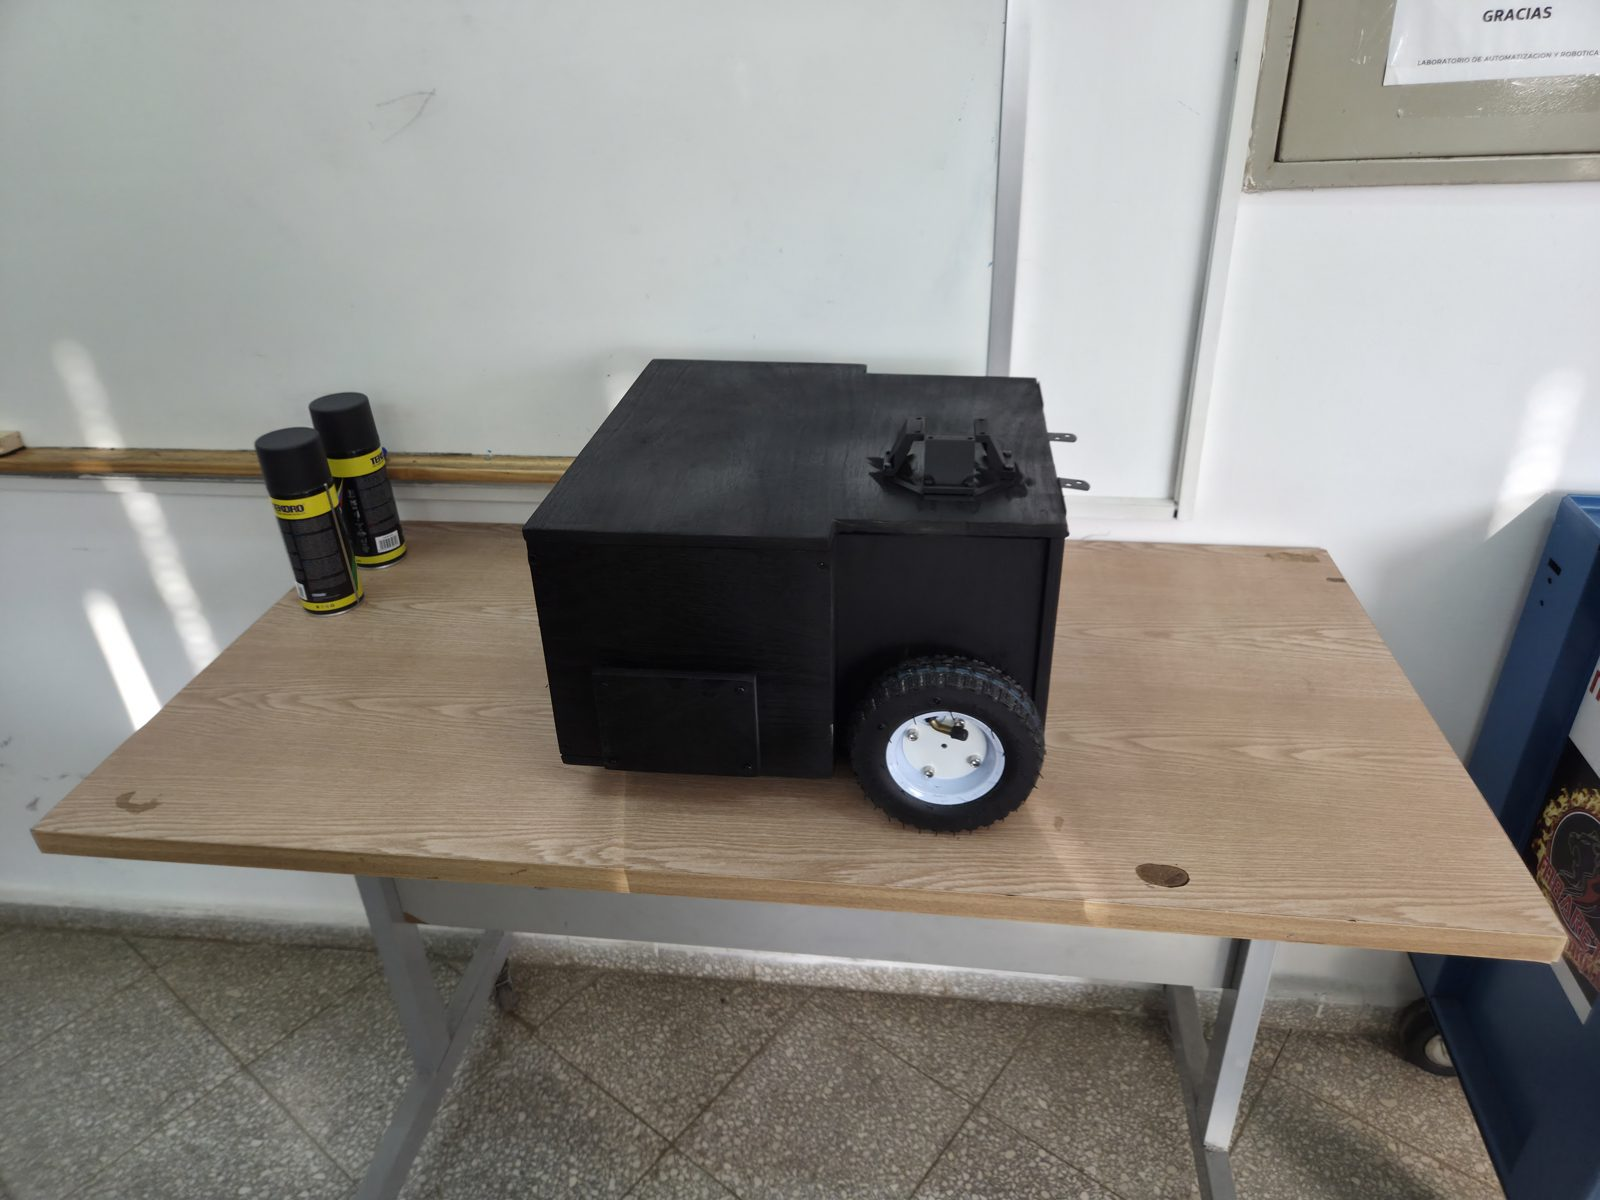
\includegraphics[width=\linewidth]{robot_izq.jpg}\caption{Vista lateral.}\end{subfigure}
\caption{La base de madera (entrega R2~E3).}
\end{figure}

\section{Tracción diferencial}

\subsection{Cómo se mueve un robot diferencial}
El robot tiene \textbf{dos ruedas motrices independientes} sobre el mismo eje y dos ruedas locas que solo apoyan.
No tiene dirección: para girar, una rueda va más rápido que la otra.

\begin{figure}[H]
\centering
\begin{tikzpicture}[scale=1.1]
  \draw[thick,fill=suave] (-1.2,-1) rectangle (1.2,1.4);
  \fill[tinta] (-1.45,-0.45) rectangle (-1.2,0.45); \fill[tinta] (1.2,-0.45) rectangle (1.45,0.45);
  \draw[dashed] (-1.6,0) -- (1.6,0);
  \fill[rojo] (0,0) circle (2pt);
  \draw[->,very thick,acento] (-1.33,0) -- (-1.33,1.0) node[above]{$v_i$};
  \draw[->,very thick,acento] (1.33,0) -- (1.33,1.6) node[above]{$v_d$};
  \draw[->,thick,rojo] (0,0) -- (0,1.3) node[above left]{$v$};
  \draw[->,thick,rojo] (0.5,0.2) arc (0:150:0.5) node[left]{$\omega$};
  \draw[<->] (-1.33,-1.3) -- node[below]{$b$ (trocha)} (1.33,-1.3);
  \node[align=left,anchor=west,font=\small] at (2.2,0.4) {
    $v = \dfrac{v_d + v_i}{2}$ \qquad $\omega = \dfrac{v_d - v_i}{b}$\\[10pt]
    $v_i = v - \omega\,\dfrac{b}{2}$ \qquad $v_d = v + \omega\,\dfrac{b}{2}$\\[10pt]
    $\text{rpm}_{i,d} = \dfrac{60\, v_{i,d}}{2\pi r}$};
\end{tikzpicture}
\caption{Cinemática diferencial. $v$ es la velocidad de avance del centro del eje [m/s], $\omega$ la velocidad de
giro [rad/s, positiva a la izquierda], $r = 0{,}075$~m el radio de rueda y $b = 0{,}40$~m la trocha (estimada:
\textbf{MEDIR}).}
\label{fig:diferencial}
\end{figure}

Ejemplos:
\begin{itemize}
  \item $v = 0{,}10$~m/s, $\omega = 0$: las dos ruedas a $\frac{60 \cdot 0{,}10}{2\pi \cdot 0{,}075} \approx 12{,}7$~rpm. Avanza recto.
  \item $v = 0$, $\omega = 0{,}5$~rad/s: $v_d = +0{,}10$, $v_i = -0{,}10$~m/s. Gira sobre su eje hacia la izquierda.
  \item $v = 0{,}10$, $\omega = 0{,}25$: $v_d = 0{,}15$, $v_i = 0{,}05$~m/s. Avanza curvando a la izquierda con radio
        $v/\omega = 0{,}4$~m.
\end{itemize}

Esto es lo que hace la clase \cod{Diferencial} del firmware de la base (\archivo{firmware/base/lib/BaseLogica/}): recibe
$(v, \omega)$ de \topic{/cmd\_vel}, calcula las rpm de cada rueda y, si alguna supera el máximo, \textbf{reduce las dos
en la misma proporción} para conservar la curvatura (el robot hace la misma curva, más despacio). Además aplica una
\textbf{rampa}: la velocidad cambia como mucho 0,3~m/s² y 1,5~rad/s², para que el robot no pegue tirones.

\subsection{Ruedas y motores de tracción}

\begin{figure}[H]
\centering
\begin{subfigure}{0.26\textwidth}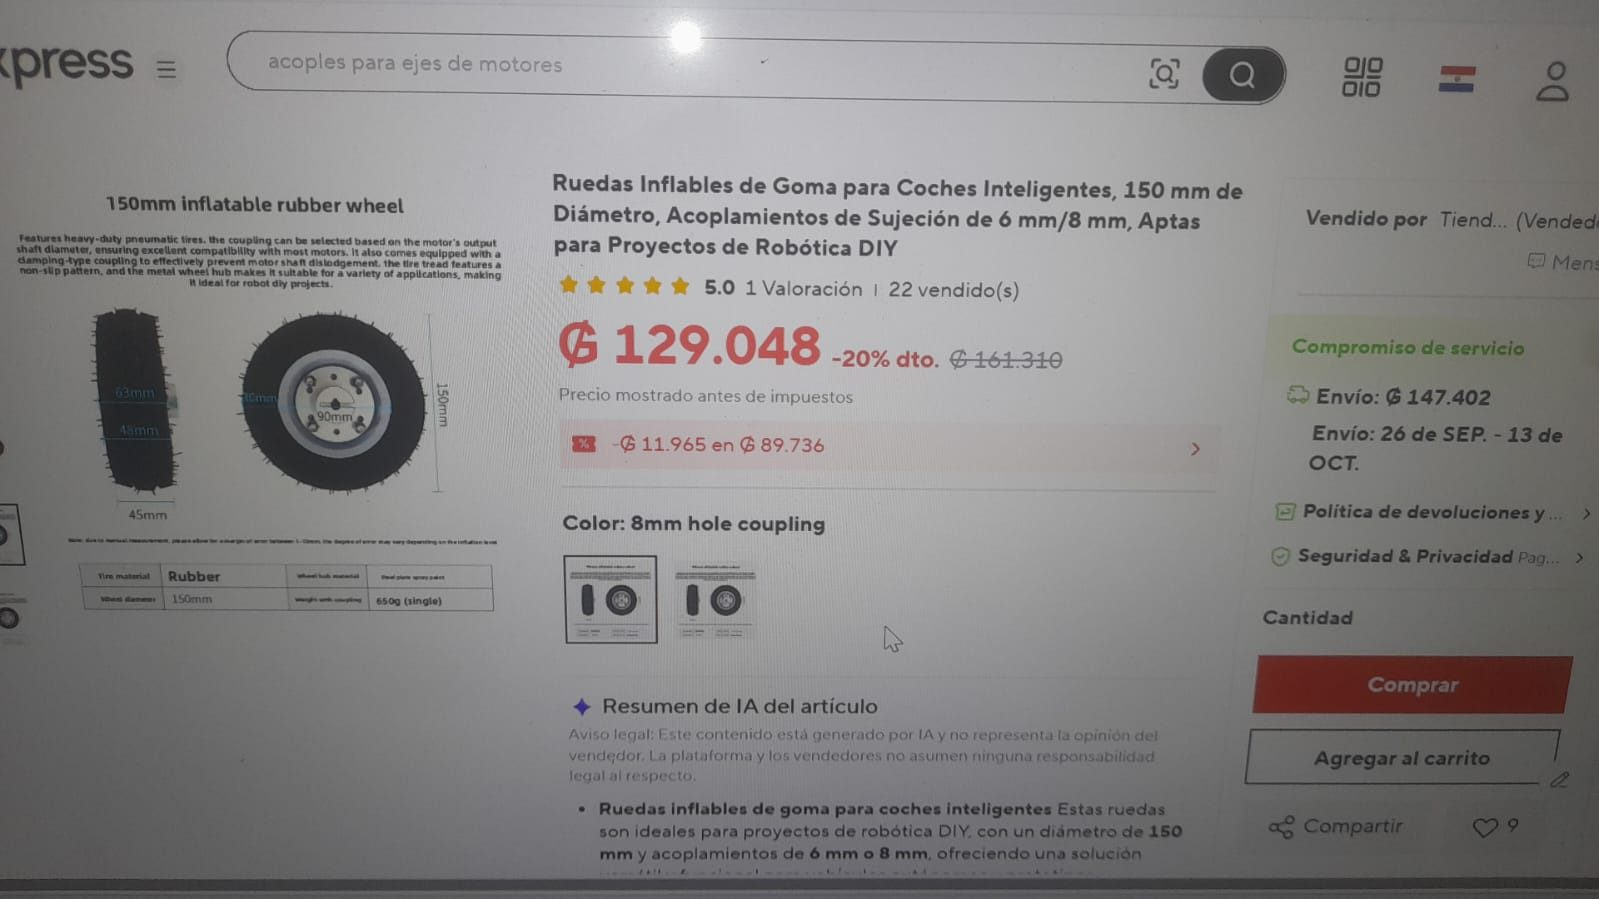
\includegraphics[width=\linewidth]{rueda.jpg}\caption{Rueda inflable de 150 mm.}\end{subfigure}\hfill
\begin{subfigure}{0.26\textwidth}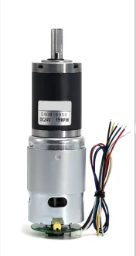
\includegraphics[width=\linewidth]{p_motor_traccion.jpg}\caption{42GM-895H con encoder.}\end{subfigure}\hfill
\begin{subfigure}{0.44\textwidth}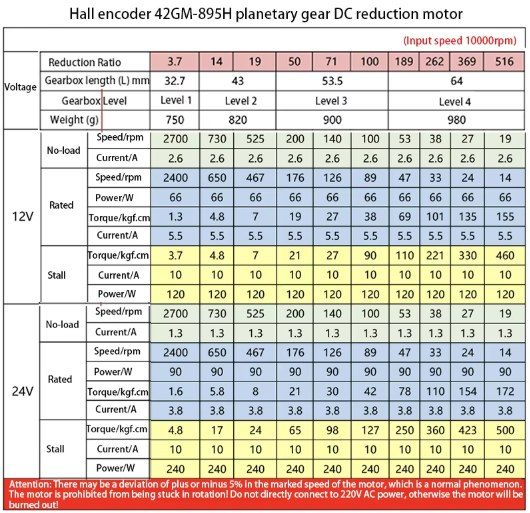
\includegraphics[width=\linewidth]{tabla_42gm.jpg}\caption{Hoja del vendedor (columna 189).}\end{subfigure}
\caption{Ruedas y motores de tracción.}
\end{figure}

\begin{center}
\begin{tabular}{@{}ll@{}}
\toprule
\textbf{Dato} & \textbf{Valor} \\
\midrule
Rueda & inflable, 150~mm de diámetro, 45~mm de ancho, 650~g \\
Motor & 42GM-895H planetario, 12~V, reducción 189:1 \\
Velocidad sin carga / nominal & 53~rpm / 47~rpm \\
Par nominal / trabado & 69~kgf·cm / 110~kgf·cm \\
Corriente sin carga / nominal / trabado & 2,6~A / 5,5~A / 10~A \\
Encoder & Hall, 11 pulsos por vuelta del motor, canales A y B, alimentado a 5~V \\
Cuentas por vuelta de la rueda & $11 \times 4 \times 189 = 8316$ (cuadratura ×4) \textbf{MEDIR} \\
Velocidad máxima teórica & $53 \cdot \pi \cdot 0{,}15 / 60 \approx 0{,}42$~m/s \\
Velocidad máxima configurada & 0,25~m/s y 1~rad/s (\cod{CFG\_DIF} en \archivo{base\_config.h}) \\
Velocidad de crucero del recorrido & 0,10~m/s \\
\bottomrule
\end{tabular}
\end{center}

\begin{nota}[Por qué se cuentan 4 flancos]
El encoder tiene dos canales, A y B, desfasados un cuarto de período. Contando los flancos de subida y de bajada de
los dos canales se obtienen 4 cuentas por pulso (``cuadratura ×4''), y el orden en que cambian A y B dice el
sentido de giro. El PCNT del ESP32 hace esto por hardware.
\end{nota}

\section{El brazo}

\subsection{Tipo y geometría}
El brazo es un manipulador \textbf{RRR} (tres articulaciones rotativas) del tipo \textbf{uArm / Dobot Magician}:
\begin{itemize}
  \item \textbf{J1 (base)} gira todo el brazo alrededor de un eje vertical.
  \item \textbf{J2 (hombro)} levanta la barra principal $L_2$.
  \item \textbf{J3 (codo)} mueve, a través de un \textbf{mecanismo de cuatro barras}, el antebrazo $L_3$. El motor
        de J3 está abajo, en la base del brazo, no en el codo: así el brazo es más liviano.
  \item Un \textbf{paralelogramo} mantiene la herramienta \textbf{siempre horizontal}, apuntando hacia afuera en
        la dirección de J1. Por eso basta con 3 motores para posicionar la pinza.
\end{itemize}

\begin{figure}[H]
\centering
\begin{tikzpicture}[scale=0.85]
  \fill[suave] (-1.5,-0.3) rectangle (1.5,0); \draw (-1.5,0) -- (1.5,0);
  \draw[very thick] (0,0) -- (0,1.5) node[midway,left]{$H_1 = 150$};
  \fill[tinta] (0,1.5) circle (3pt);
  \coordinate (B) at ($(0,1.5)+(50:3.5)$);
  \draw[line width=3pt,verde] (0,1.5) -- (B) node[midway,above left]{$L_2 = 350{,}2$};
  \fill[tinta] (B) circle (3pt);
  \coordinate (P) at ($(B)+(-20:3.3)$);
  \draw[line width=3pt,acento] (B) -- (P) node[midway,above right]{$L_3 = 329{,}5$};
  \fill[tinta] (P) circle (3pt) node[below]{muñeca $P_3$};
  \draw[line width=2pt,naranja] (P) -- ++(0.9,0) node[right]{TCP};
  \draw[dashed,gris] (0,1.5) -- (3,1.5);
  \draw[->] (1.2,1.5) arc (0:50:1.2) node[midway,right]{$q_2$};
  \draw[dashed,gris] (B) -- ($(B)+(50:1.5)$);
  \draw[->] ($(B)+(50:1.0)$) arc (50:-20:1.0) node[midway,right]{$q_{3O}$};
  % cuatro barras simplificado
  \draw[thick,rojo] (0,1.5) -- ++(-40:0.6) coordinate (r1);
  \draw[thick,ocre] (r1) -- ($(B)+(-110:0.6)$) node[midway,right,font=\scriptsize]{$L_4 = 338$};
  \draw[thick,rojo] (B) -- ($(B)+(-110:0.6)$);
  \node[font=\scriptsize,rojo] at (-0.2,0.85) {balancín};
  \draw[->,thick] (-1.0,0.3) arc (200:340:1.0 and 0.3) node[right]{$q_1$};
  \node[align=left,font=\small,anchor=west] at (6.6,2.6) {Medidas en mm (entrega R1~E4):\\
    $H_1 = 150$ (altura del hombro)\\ $L_2 = 350{,}22$ (barra verde)\\ $L_3 = 329{,}51$ (antebrazo)\\
    $L_4 = 338$ (acoplador)\\ $L_{3,0} = L_{3,1} = 40$ (balancines)\\[4pt]
    Rangos:\\ $q_1 \in [45^\circ, 225^\circ]$\\ $q_2 \in [-25^\circ, 135^\circ]$\\ $q_3 \in [-50^\circ, 50^\circ]$};
\end{tikzpicture}
\caption{Esquema lateral del brazo (no a escala). El motor de J3 mueve el balancín rojo de abajo; el acoplador
amarillo transmite el movimiento al codo. $q_{3O}$, el ángulo del antebrazo respecto de la prolongación de $L_2$, es
una consecuencia de $q_2$ y $q_3$ por el cierre del cuatro barras.}
\label{fig:brazo}
\end{figure}

\begin{pendiente}[Balancín del cuatro barras]
\archivo{cinematica.py} usa balancines de 40~mm (E4). Según \archivo{ARQUITECTURA.md} §11, el balancín rojo se
cambió a \textbf{60~mm} el 03/10 para que el mecanismo sea de Grashof. Verificar la medida real y, si cambió,
actualizar \cod{L30} en \archivo{ros2\_ws/src/brazo\_ik/brazo\_ik/cinematica.py} y volver a correr sus pruebas.
\end{pendiente}

\subsection{Dónde va montado y qué alcanza}
El brazo va \textbf{atrás a la izquierda, sobre el eje de tracción}, a unos 6~cm del costado ($y = 0{,}11$~m,
preliminar). $q_1 = 0$ apunta hacia adelante y crece en sentido antihorario visto desde arriba. El rango de J1
($45^\circ$ a $225^\circ$) va de adelante-izquierda, pasando por la izquierda y por atrás, hasta atrás-derecha: \textbf{nunca
cruza el mástil de las cámaras}, que está adelante a la derecha. $q_1 = 90^\circ$ (brazo hacia el costado izquierdo) es
la marca del banco de pruebas y la pose de cero de J1.

La consigna de R1 define la zona de trabajo como una esfera de 30~cm de diámetro centrada a unos 35~cm del suelo.
Con el robot centrado en el pasillo de la simulación, los limones quedan a unos 0,45~m del eje de J1.

\subsection{Motores y transmisiones}

\begin{center}
\begin{tabular}{@{}lccc@{}}
\toprule
 & \textbf{J1 (base)} & \textbf{J2 (hombro)} & \textbf{J3 (codo)} \\
\midrule
Motor & 36GP-555, 160~rpm & 36-555, 58~rpm & 36-555, 58~rpm \\
Reductora del motor & 50:1 & 139:1 & 139:1 \\
Transmisión & correa GT2 18 → 90 (5:1) & helicoidales 15 → 75 (5:1) & helicoidales 15 → 75 (5:1) \\
Velocidad máx. de la articulación & 32~rpm (192~°/s) & 11,6~rpm (70~°/s) & 11,6~rpm (70~°/s) \\
Encoder & \multicolumn{3}{c}{SCX-555, 16 pulsos por vuelta, cuadratura ×4, alimentado a \textbf{3,3~V}} \\
Cuentas por vuelta de la articulación & $3200 \times 5 = 16\,000$ & $8896 \times 5 = 44\,480$ & $44\,480$ \\
Resolución & 44,4 cuentas/° & 123,6 cuentas/° & 123,6 cuentas/° \\
Corriente (vacío / nominal / trabado) & \multicolumn{3}{c}{0,5~A / 1,3~A / 10~A a 12~V} \\
Se autobloquea & no & \textbf{no} & \textbf{no} \\
Estado & medido (02/10) & llega 19--29/10 & llega 19--29/10 \\
\bottomrule
\end{tabular}
\end{center}

\begin{peligro}[J2 y J3 no se sostienen solos]
Los motores planetarios de J2 y J3 \textbf{no se autobloquean}: sin corriente, el brazo cae por su peso. Pasa al
apretar la seta, al desarmar en rueda libre o al cortar los 12~V. Dejar siempre el brazo en reposo \textbf{apoyado en
un tope} y no poner las manos debajo. Falta resolver cómo sostenerlo (contrapeso o resorte con lo que haya).
\end{peligro}

\begin{figure}[H]
\centering
\begin{subfigure}{0.24\textwidth}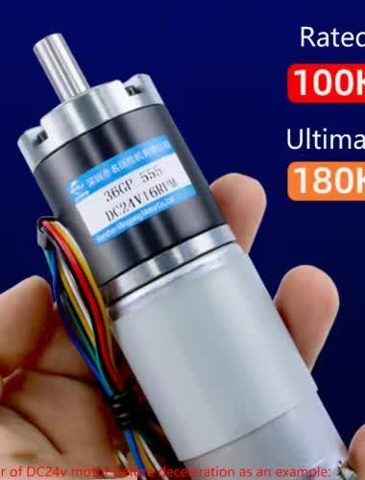
\includegraphics[width=\linewidth]{p_motor_brazo.jpg}\caption{36GP-555 con encoder.}\end{subfigure}\hfill
\begin{subfigure}{0.24\textwidth}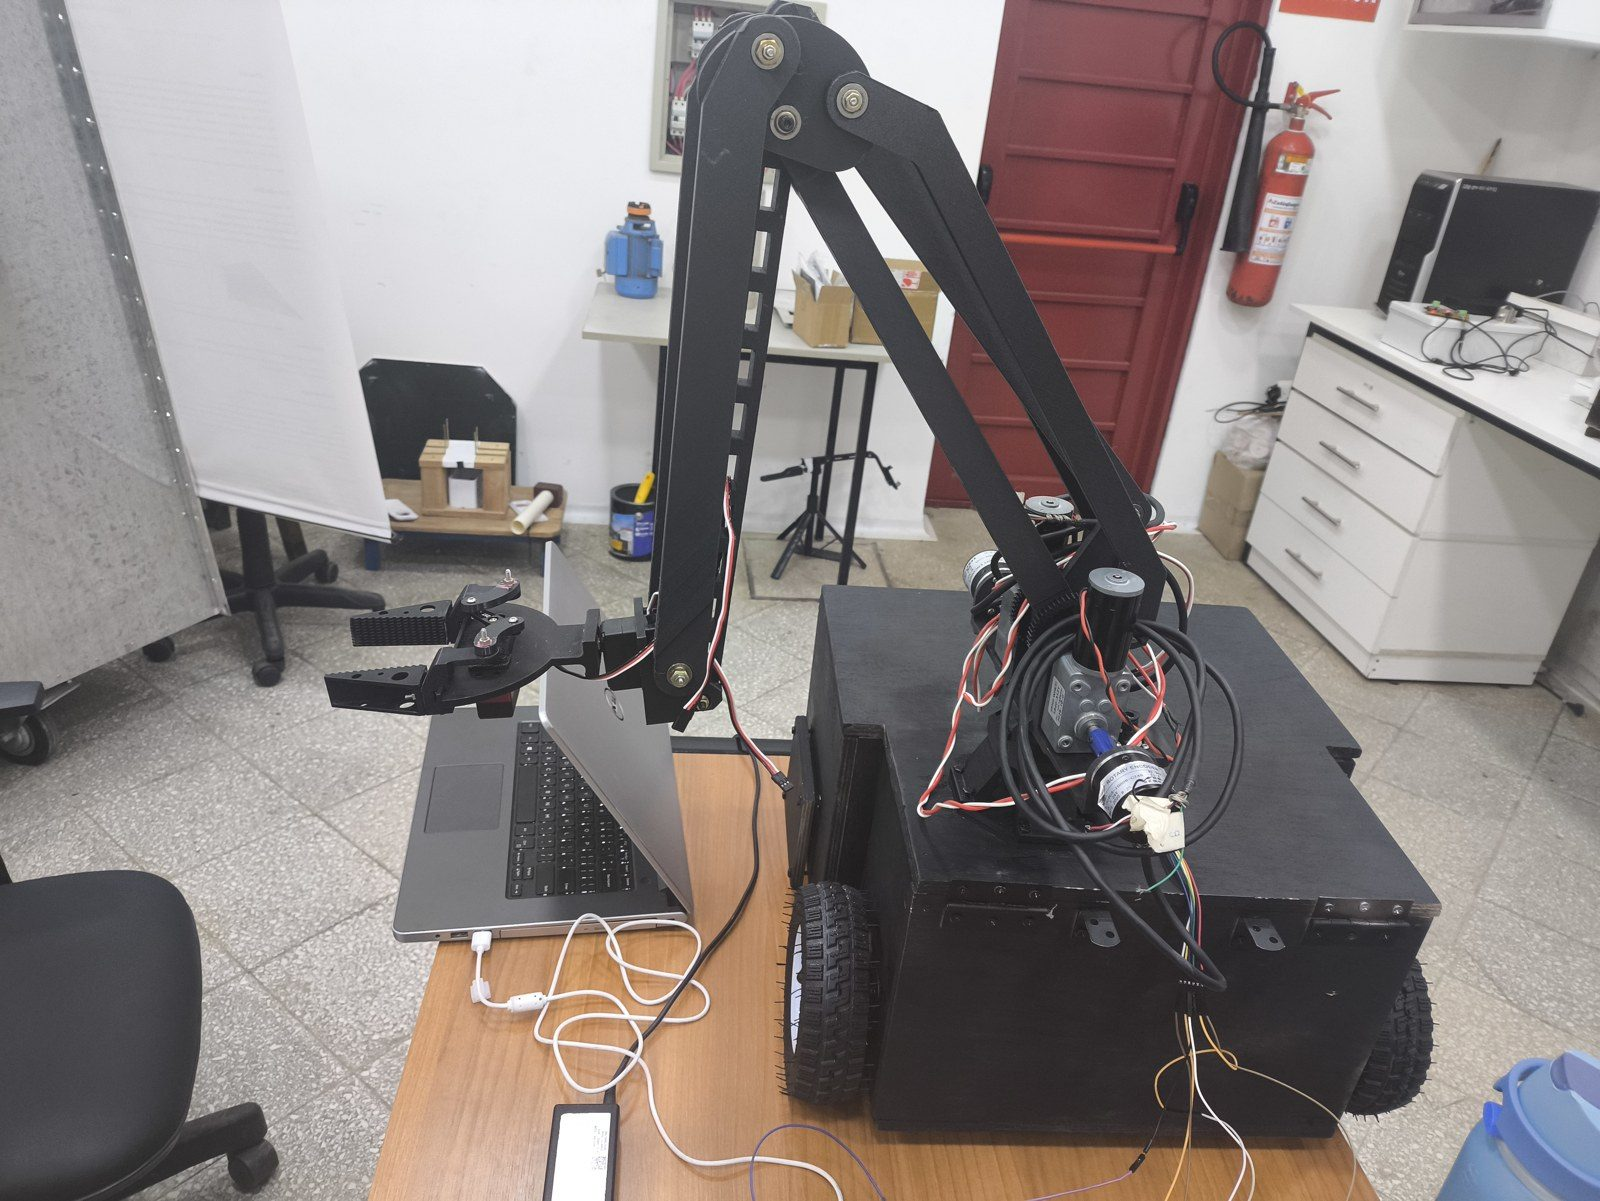
\includegraphics[width=\linewidth]{brazo_j1_cero.jpg}\caption{J1 en su cero.}\end{subfigure}\hfill
\begin{subfigure}{0.24\textwidth}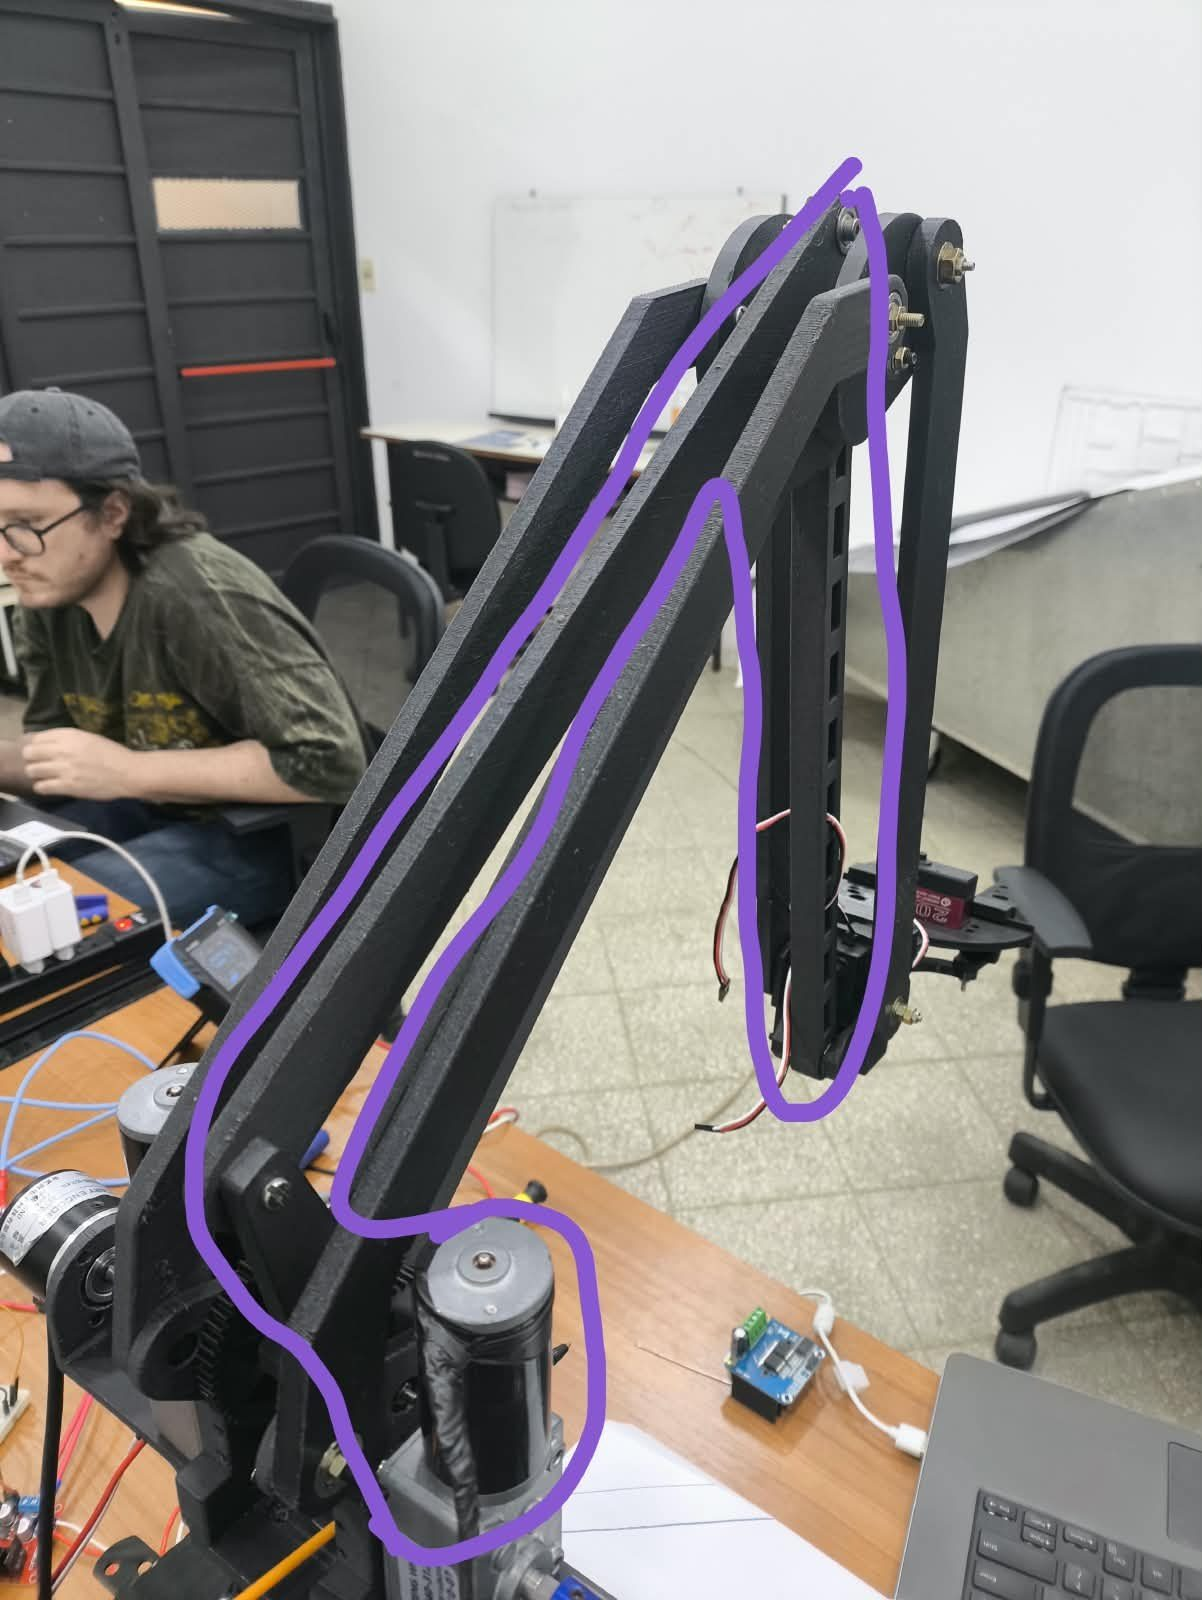
\includegraphics[width=\linewidth]{brazo_codo_j3.jpg}\caption{Cuatro barras del codo.}\end{subfigure}\hfill
\begin{subfigure}{0.24\textwidth}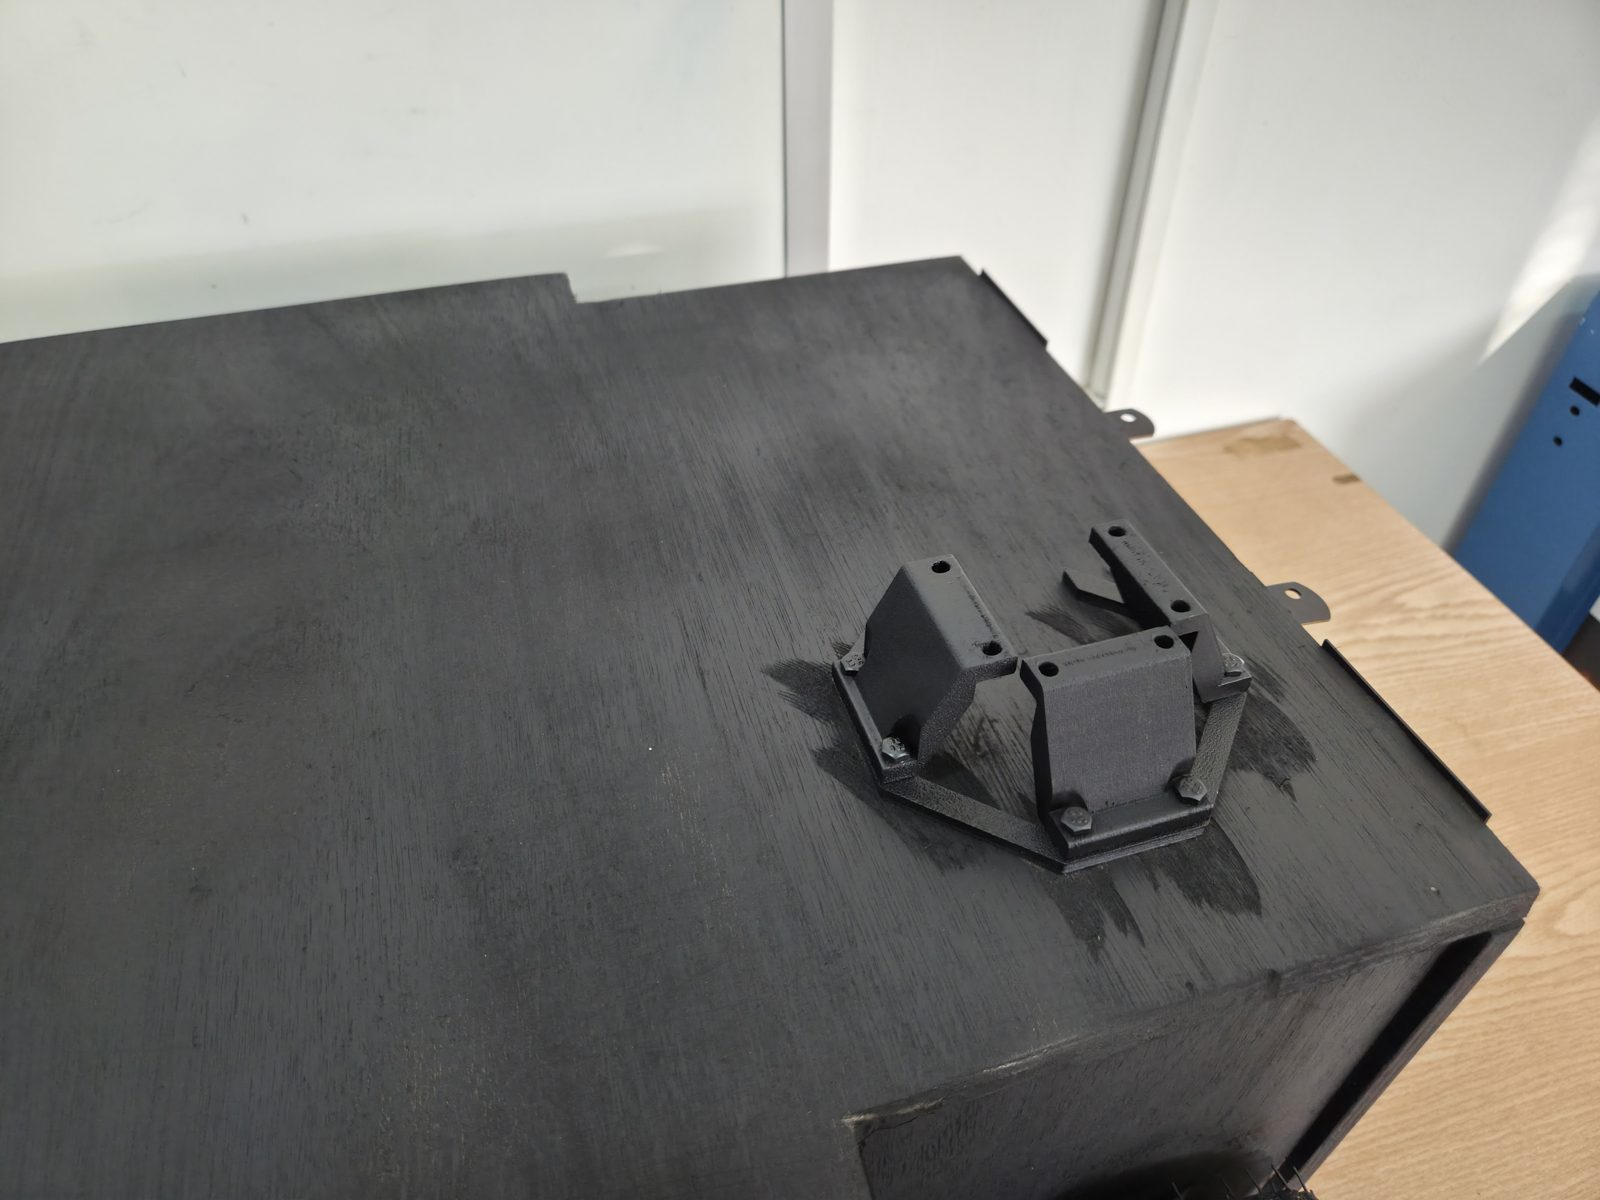
\includegraphics[width=\linewidth]{base_brazo.jpg}\caption{Base impresa del brazo.}\end{subfigure}
\caption{Motores y partes del brazo.}
\end{figure}

Colores de los cables de los 36GP-555: \textbf{blanco} = motor +, \textbf{amarillo} = motor −, \textbf{verde} =
encoder + (a 3,3~V), \textbf{azul} = GND, \textbf{negro} = canal A, \textbf{rojo} = canal B. El encoder tiene salida de
colector abierto con pull-up de 5,1~kΩ en su plaquita: alimentado a 3,3~V, sus salidas quedan en 0 o 3,3~V, que el
ESP32 tolera.

\section{La pinza}

La pinza tiene dos servos \textbf{DSSERVO RDS3218} de 20~kg·cm, alimentados con 6~V por el buck~3:
\begin{itemize}
  \item \textbf{Apertura} (GPIO~4 de la WROOM): 0~\% = abierta, 100~\% = cerrada (\topic{/pinza/cierre}).
  \item \textbf{Giro J4} (GPIO~14): rota la pinza alrededor del eje de la herramienta, de $-90^\circ$ a $+90^\circ$
        (\topic{/pinza/giro}). Sirve para desprender el limón retorciendo el pedúnculo.
\end{itemize}
La cosecha es: \textbf{agarrar} (cerrar), \textbf{traccionar} (retroceder 1--2~cm), \textbf{girar} J4 y
\textbf{retirar}. Hoy la misión hace solo agarrar y retirar; el giro queda para después.

\begin{figure}[H]
\centering
\begin{subfigure}{0.28\textwidth}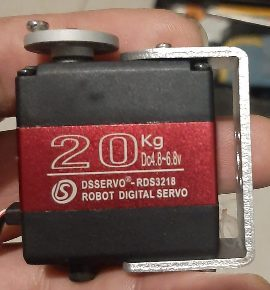
\includegraphics[width=\linewidth]{p_servo.jpg}\caption{Servo RDS3218.}\end{subfigure}\hspace{8mm}
\begin{subfigure}{0.28\textwidth}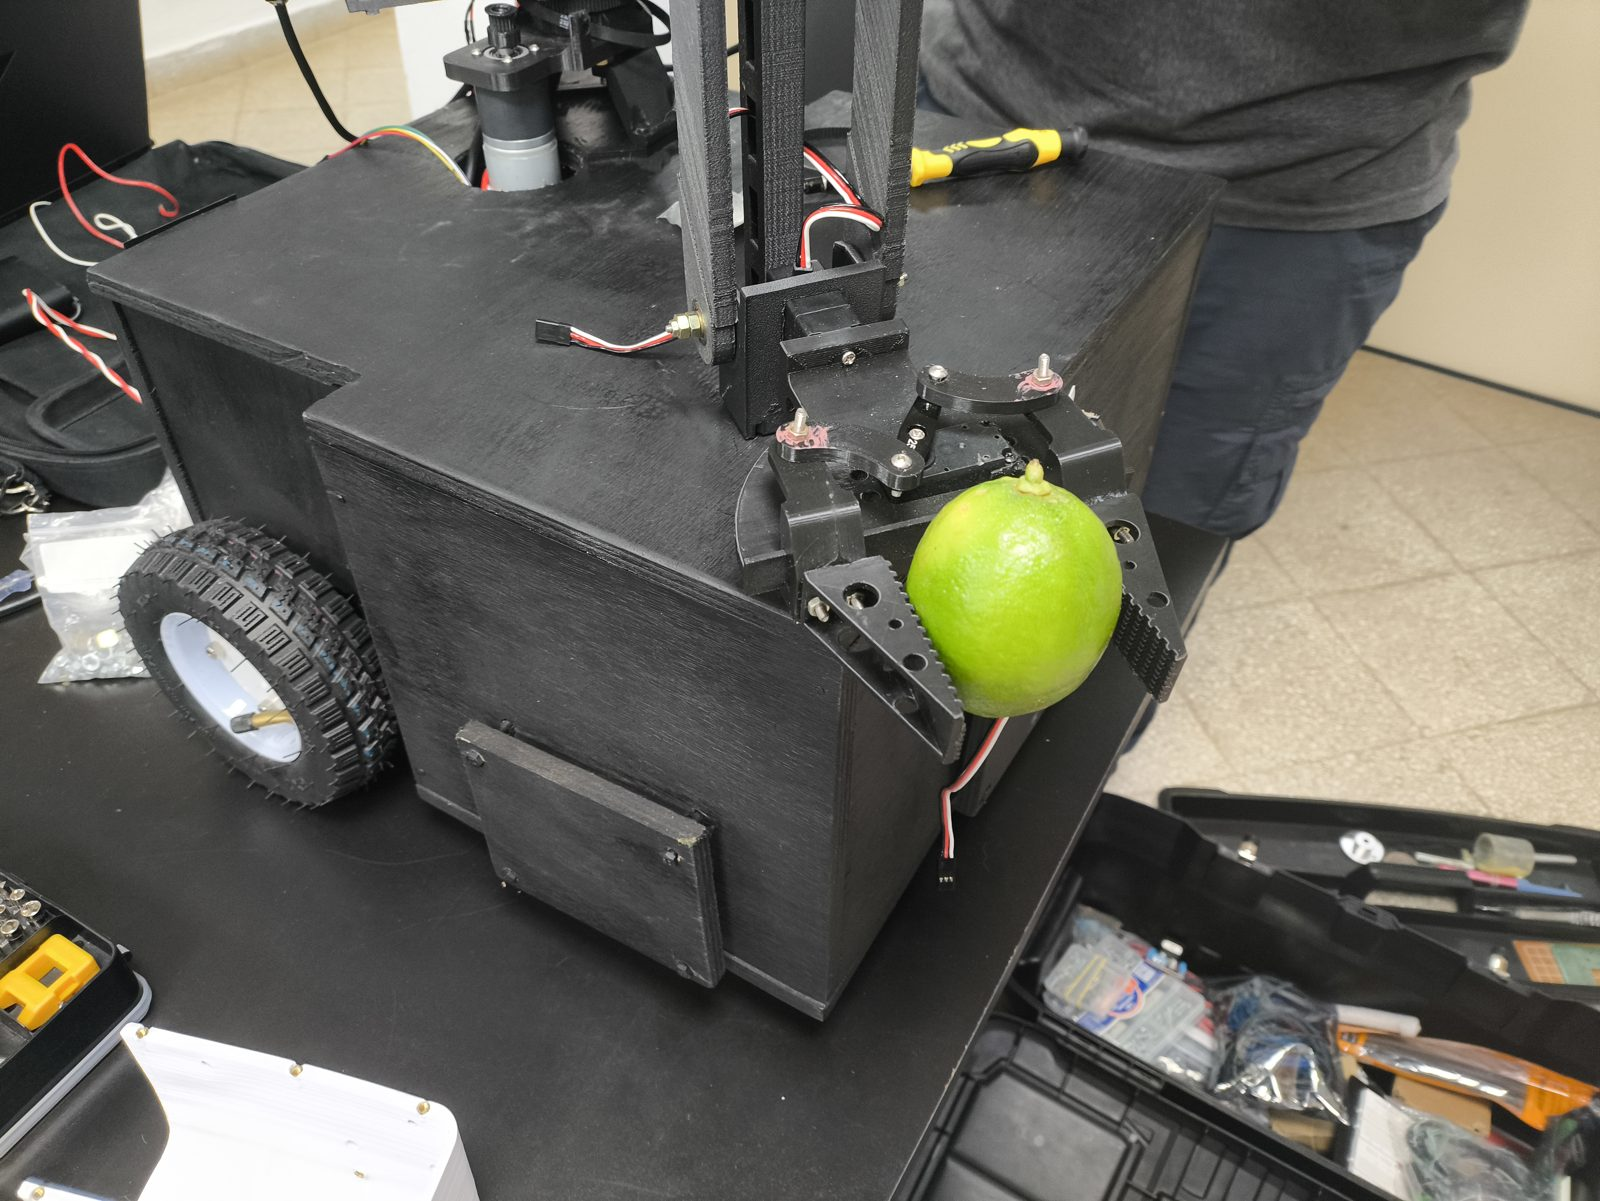
\includegraphics[width=\linewidth]{robot_limon.jpg}\caption{Pinza con un limón.}\end{subfigure}
\caption{La pinza.}
\end{figure}

\begin{pendiente}
Pulsos reales de cada servo (\cod{PINZA\_US\_*}, \cod{GIRO\_US\_*}), el porcentaje de cierre que agarra sin aplastar
(\cod{cierre} en la misión) y \cod{largo\_herramienta}: la distancia horizontal de la muñeca al centro del agarre
(capítulo~\ref{cap:ik}).
\end{pendiente}
